%
% $RCSfile: dual_model_approach.tex,v $
%
% Copyright (C) 2002-2008. Christian Heller.
%
% Permission is granted to copy, distribute and/or modify this document
% under the terms of the GNU Free Documentation License, Version 1.1 or
% any later version published by the Free Software Foundation; with no
% Invariant Sections, with no Front-Cover Texts and with no Back-Cover
% Texts. A copy of the license is included in the section entitled
% "GNU Free Documentation License".
%
% http://www.cybop.net
% - Cybernetics Oriented Programming -
%
% http://www.resmedicinae.org
% - Information in Medicine -
%
% Version: $Revision: 1.1 $ $Date: 2008-08-19 20:41:06 $ $Author: christian $
% Authors: Christian Heller <christian.heller@tuxtax.de>
%

\subsection{Dual Model Approach}
\label{dual_model_approach_heading}
\index{Dual Model Approach}
\index{Analysis Pattern}
\index{Two Level Modelling}
\index{Knowledge Level}
\index{Operational Level}
\index{Reflection Pattern}
\index{Meta Level}
\index{Base Level}
\index{Archetype Model}
\index{AM}
\index{Reference Model}
\index{RM}
\index{ADL}
\index{OpenEHR}

The idea of archetypes was inspired by Martin Fowler's \emph{Analysis Patterns}
\cite{fowler1997} describing a kind of ad hoc two-level modelling, using a
\emph{Knowledge Level} and \emph{Operational Level} -- as described by the
\emph{Reflection} pattern (section \ref{reflection_heading}), which calls the
two levels \emph{Meta Level} and \emph{Base Level}, respectively. Fowler tried
to put as much general domain knowledge as possible into the meta level, in
order to make application systems more flexible, and to remove unnecessary
dependencies. Archetypes represent what would traditionally have been put into
the knowledge (meta) level.

Because an \emph{Archetype Model} (AM) (defined in form of ADL documents) and
its runtime instances constrain a \emph{Reference Model} (RM) and its instances
(figure \ref{dual_figure}), development with archetypes is called the
\emph{Dual Model Approach} \cite{openehr}. Archetypes represent the knowledge
belonging to the meta level; the reference model contains information belonging
to the base level. \textit{RMs are domain-invariant, i.e. the concepts
expressed in the base models mean the same thing right across the domain.}
\cite[Beale]{openehrtechnical}

\begin{figure}[ht]
    \begin{center}
        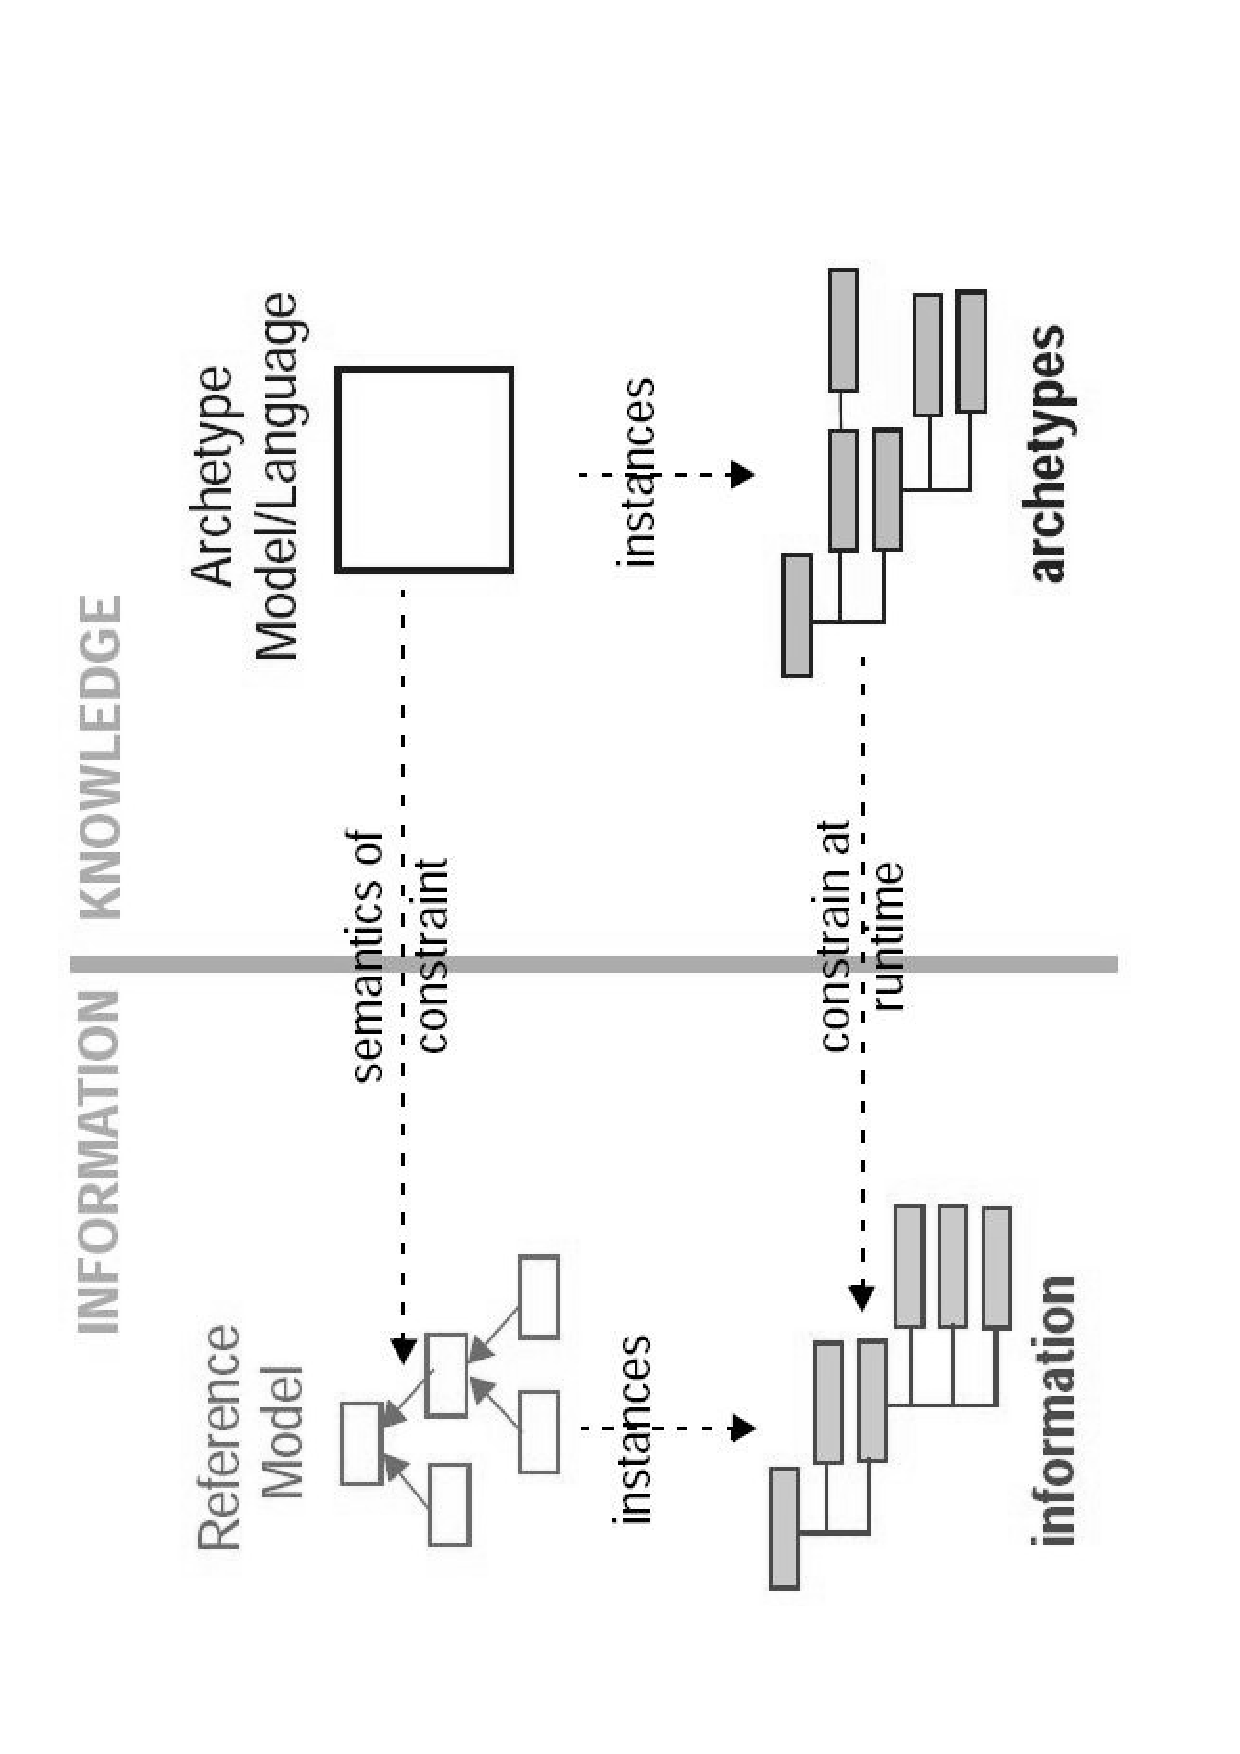
\includegraphics[scale=0.3,angle=-90]{graphic/dual.pdf}
        \caption{Dual Model Approach \cite{archetypes}}
        \label{dual_figure}
    \end{center}
\end{figure}

The difference between the dual model approach and classical meta architectures
is that the latter implement both, meta- and base level using the same
technology (language). Archetypes, on the other hand, use the ADL for
specifying knowledge. Further, the AM does not depend on the RM, as opposed to
meta architectures, where both models depend on each other bidirectionally.
Ergo, the dual model approach is rather comparable to \emph{Agents} (section
\ref{agent_oriented_programming_heading}) owning a mental state (knowledge base).

There are unclear views on what exactly should be constrained when. Sam Heard
\cite{openehrtechnical} writes about an \emph{Archetype Kernel} -- a tool that
could help build (knowledge instances) and ensure that (they) comply to
archetypes \ldots\ It could operate at a range of points, at:

\begin{itemize}
    \item[a] write and edit time: allowing constraint of the data to be based
        on archetypes (metadata) rather than application specific processes;
    \item[b] creation time of the application or schema: so that the
        application has read all information constraining the data as indicated
        -- but not through interaction with the archetype at runtime;
    \item[c] persistence time: into a database or some other persistence means;
    \item[d] communication time: such as when creating a model extract.
\end{itemize}

Besides obvious benefits of these approaches in constraining domain knowledge,
there are a number of potential problems, as Heard mentions:

\begin{quote}
    \emph{a} makes \emph{b} and \emph{c} redundant and allows the application
    to stay up to date with the archetype development process; \emph{b} makes
    \emph{c} redundant (potentially) but means code has to be cut to
    encorporate new archetypes; \emph{c} and \emph{d} mean that data may be
    proved incompatible at a time later than data entry and this may lead to
    other problems; \emph{d} means you can carry on regardless but there is a
    risk that data collected will not be compatible with models that are
    proposed for interoperability.
\end{quote}

Further weaknesses of archetypes, the ADL and dual model approach are:

\begin{itemize}
    \item[-] mix of meta information (properties, constraints) and hierarchical whole-part structure in ADL
    \item[-] incomplete domain knowledge in ADL lacking logic (algorithms/ workflows) and user interfaces
    \item[-] inflexible structures due to runtime-dependency of RM instances from archetypes
    \item[-] use of object-oriented concepts with all their limits, for RM as well as for AM instances
\end{itemize}

Although the \emph{OpenEHR} project \cite{openehr} claims archetypes to be both:

\begin{enumerate}
    \item[-] \emph{domain-empowered:} domain experts, rather than information
        technology people, become able to directly define and manage the
        knowledge definitions of their systems;
    \item[-] \emph{future-proof:} systems can be deployed prior to having
        created formal knowledge models of the (entire) domain
\end{enumerate}

\ldots\ the above-mentioned issues prevent them from being so. The dual model
approach in conjunction with archetypes only partly fulfills the expectations
of independent and complete knowledge structures. CYBOP sets out to solve these
issues and to find a truely future-proof, long-life system architecture.
Knowledge templates written in the language described later in this work
(chapter \ref{cybernetics_oriented_language_heading}) may not only contain meta
information constraining application models (as archetypes do), they represent
the application itself. The templates themselves are constrained at design time
through one universal knowledge schema (chapter \ref{knowledge_schema_heading})
dictating their structure. Runtime knowledge models do not reference the
template they were instantiated with (contrary to RM instances referencing
their corresponding AM instance); a CYBOP application holds all constraints
directly in its knowledge models (runtime instances). Since these models follow
the structure of the singular knowledge schema as well, they can be serialised
easily what makes further constrain activities for persistence or communication
unnecessary.
